% ==== Backup ====
\section*{Backup}

\begin{frame}[fragile]{Debugging / Profiling of JIT'ed code: HOWTO}
  Cling also allows debugging JITed code and offers integration with Linux's \texttt{perf}, e.g.
  \vfill

  \begin{itemize}
  \item A breakpoint on interpreted code can be set and step-into after each statement
    \begin{lstlisting}[style=bash]
$ export CLING_DEBUG=1
$ gdb --args cling /tmpl/simple.C
(gdb) break simple
(gdb) r
Starting program: cling /tmp/simple.C

Breakpoint 1, simple () at /tmp/simple.C:4
4	  std::cout << "Hello, world!" << std::endl;
(gdb) q
    \end{lstlisting}

  \item It can generate a symbol file for \texttt{perf} -- Can be used together with Flamegraph%
    \footnote{Flamegraph: \url{\flamegraphURL}}!
    \begin{lstlisting}[style=bash]
$ export CLING_PROFILE=1
$ perf record -g -e cycles -- cling /tmp/simple.C
    \end{lstlisting}
  \end{itemize}
\end{frame}

\begin{frame}{Debugging / Profiling of JIT'ed code: flamegraph}
  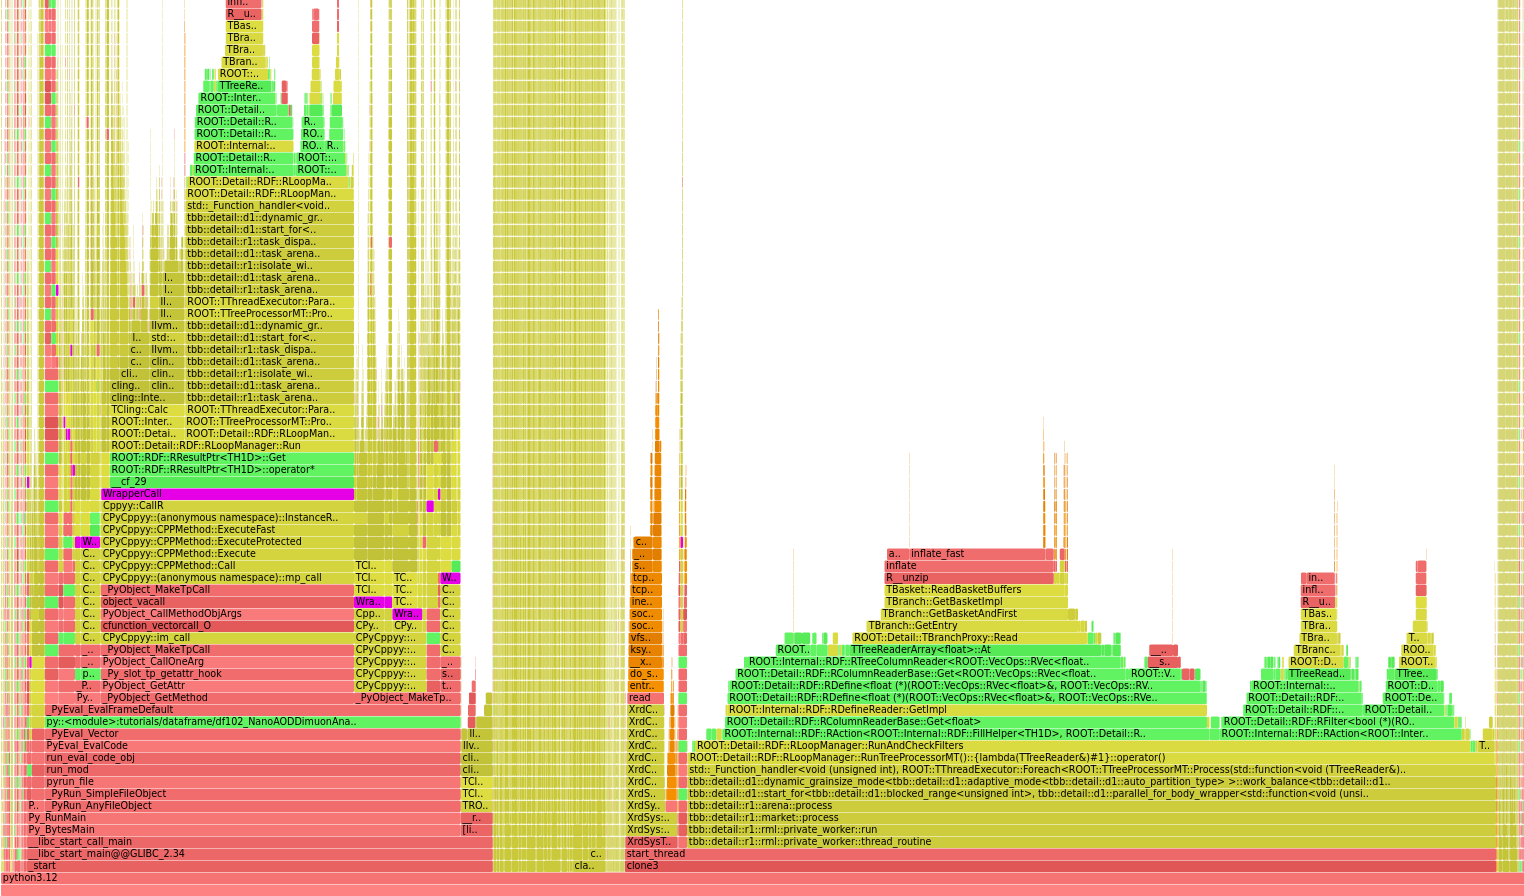
\includegraphics[width=\textwidth]{img/flamegraph-df102py3.12.png}
\end{frame}
